Due to the small mass of electron, it tends to Bremsstrahlung radiation and energy decay in the tracker system.
Electrons are expected to generate a sequence of short tracks in the tracker system under the standard tracking algorithm.
The track segments, ECAL cluster for both the track-cluster linking, and photon tracks from Bremsstrahlung are masked from the ingredient list if the considered compatible to reconstruct into a particle-flow electron.
The following section will introudce the electron reconstruction and identification in the CMS experiment.

\subsection{Electron reconstruction}
The electron tracks give information for precise momentum measurement and to distinguish electrons from photons.
However, electrons can interact with inner tracker materials and ECAL crystals producing situations such as Bremsstrahlung and conversions, as shown in Fig.~\ref{fig:reco_el_track}.
The connection and integration process between these situations can be summarized in the following parts.

\begin{figure}\centering
    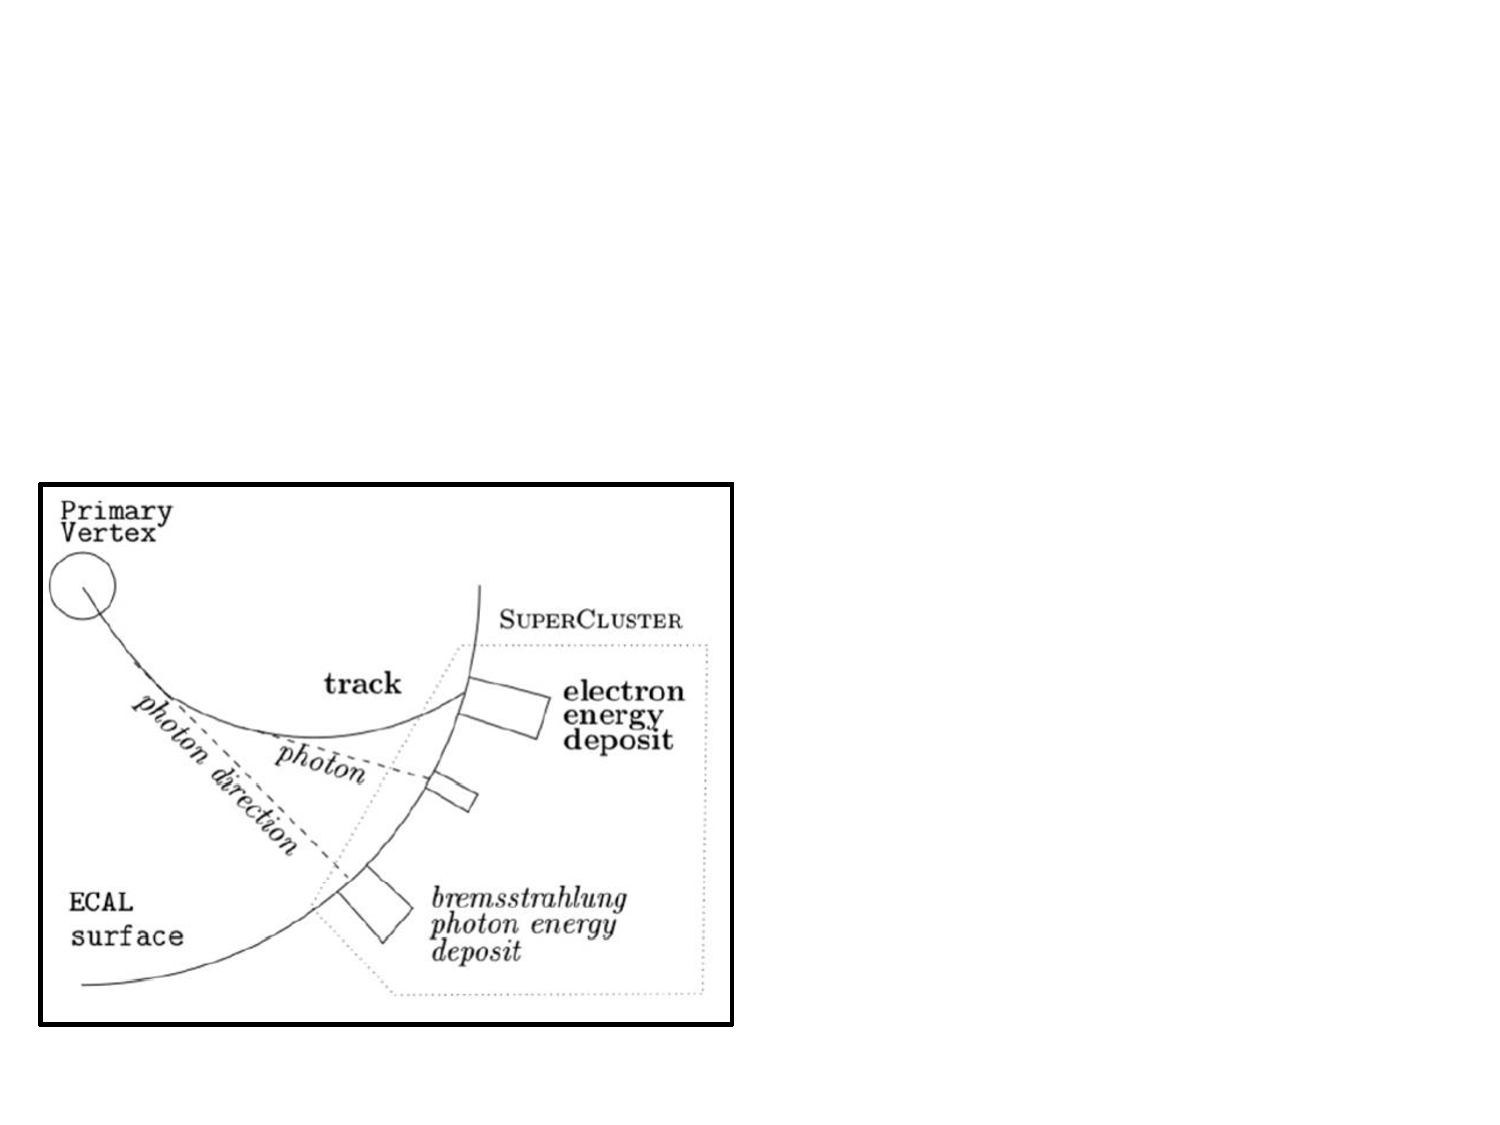
\includegraphics[width=0.75\textwidth]{figure/reco_el_track.pdf}
    \caption
    {
    Overview of an event with an electron including Bremsstrahlung tangent under the ECAL surface.
    }
    \label{fig:reco_el_track}
\end{figure}

The electron reconstruction begins with the EM supercluster reconstruction in the ECAL given by the PF cluster algorithm.
Since the Bremsstrahlung and photon conversion mainly happen with original electrons or photons from interaction points before hitting on the ECAL detector.
An ECAL cluster is not able to recover the energy of the original electrons.
The construction with supercluster, combining the associated ECAL clusters into a signal cluster, adopts a mustache algorithm to include the information from the ECAL and preshower detectors.
This algorithm starts from a seed cluster above a given threshold with additional clusters located in a mustache-like region in the $\eta-\phi$ plane (Fig.~\ref{fig:reco_beard}) to form a supercluster.
The clusters under the strong magnetic filed can then be collected under this design.

\begin{figure}\centering
    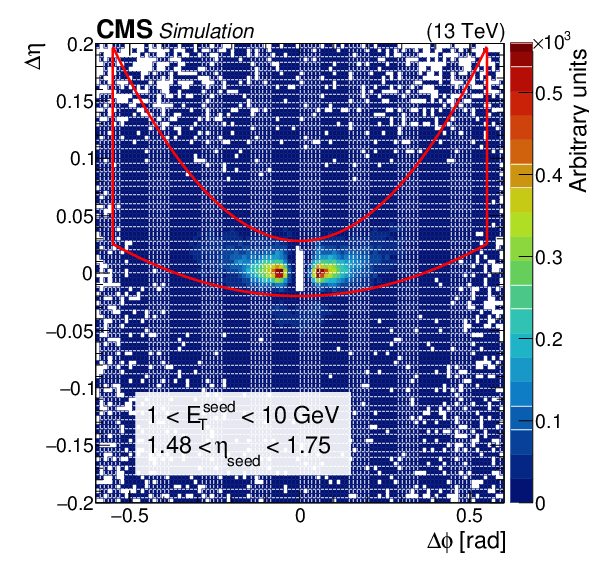
\includegraphics[width=0.55\textwidth]{figure/reco_beard.png}
    \caption[Distribution of $\Delta\eta$ versus $\Delta\phi$ for simulated electrons.]
    {
        Distribution of $\Delta\eta=\eta_{\mathrm{seed-cluster}}-\eta_{\mathrm{cluster}}$ versus $\Delta\phi = \phi_{\mathrm{seed-cluster}}  - \phi_{\mathrm{cluster}}$ for simulated electrons with $1 < \ET^{\mathrm{seed}} < 10 \GeV$ and $1.48 < \eta_{\mathrm{seed}} < 1.75$.
        The $z$-axis represents the occupancy of the number of PF clusters matched with the simulation (requiring to share at least $1\%$ of the simulated electron energy) around the seed. 
        The red line contains approximately the set of clusters selected by the mustache algorithm. 
        The white region at the center of the plot represents the $\eta-\phi$ footprint of the seed cluster.
    }
    \label{fig:reco_beard}
\end{figure}

The electrons are also reconstructed by track reconstruction in the CMS experiment.
To account for the electron energy loss from Bremsstrahlung at each layer of material, the electron tracks can be obtained after refitting the track segments with a Gaussian-sum filter (GSF) instead of the normal KF algorithm. 
The GSF track reconstruction begins with electron trajectory with either ECAL-driven seeding or tracker-driven seeding.
The ECAL-driven seeding chooses mustache clusters with $E_{\mathrm{SC,T}} > 4 \GeV$ and $H/E_{\mathrm{SC}} < 0.15$, where $E_{\mathrm{SC,T}}$ and $E_{\mathrm{SC}}$ are the transverse energy and total energy of the superclusters and $H$ indicates the HCAL tower energy deposited in $\Delta R < 0.15$ with the supercluster positions as the center.
Based on the assumption of the trajectory in a helix structure and no radiative emission, the trajectory is extrapolated to the collision vertex with the energy-weighted position, transverse energy and the magnetic filed in each selected supercluster.
The seed are considered as a electron track seed if the first two hits are matched to the extrapolated trajectory in the pixel layers or endcap tracker.
The tracker-driven seeding, in contrast, uses all inner tracks information.
The inner track seed is considered as a GSF track seed if a inner track is matched to an ECAL cluster with some track quality criteria.
Both of the seeds are then grouped together as the start point of the electron track reconstruction.
The GSF fit adopts a sum of multi-gaussian functions (as an approximation of the Bethe-Heitler formula) to estimate the parameters of the electron trajectories.

The superclusters and GSF tracks will be integrated together and the mustache superclusters will be associated with a GSF track once they are fully reconstructed.
The conversion vertexes and the associated tracks are made with information from the inner tracks, ECAL-seeded tracks and a kinematic vertex fitter.
The Bremsstrahlung photons are reconstructed by connecting the GSF tracks to the corresponding ECAL clusters via a Bremsstrahlung tangent, a extrapolated straight line.
The superclusters or the GSF tracks are connected with those conversion tracks and Bremsstrahlung tangents.
The ECAL clusters linked to both tracks are added to mustache superclusters to form refined superclusters.

Eventually, all the clusters and tracks are grouped together to form $\Pe/\gamma$ hypotheses.
The electron candidates, filter by loose criteria based on the BDT classifier to eliminate the fake ones from jet fragmentation and hadronization, is defined as an $\Pe/\gamma$ object.
The electron reconstruction efficiencies measured in 2017 data and in simulated DY samples are shown in Fig.~\ref{fig:reco_el_eff}.

\begin{figure}\centering
    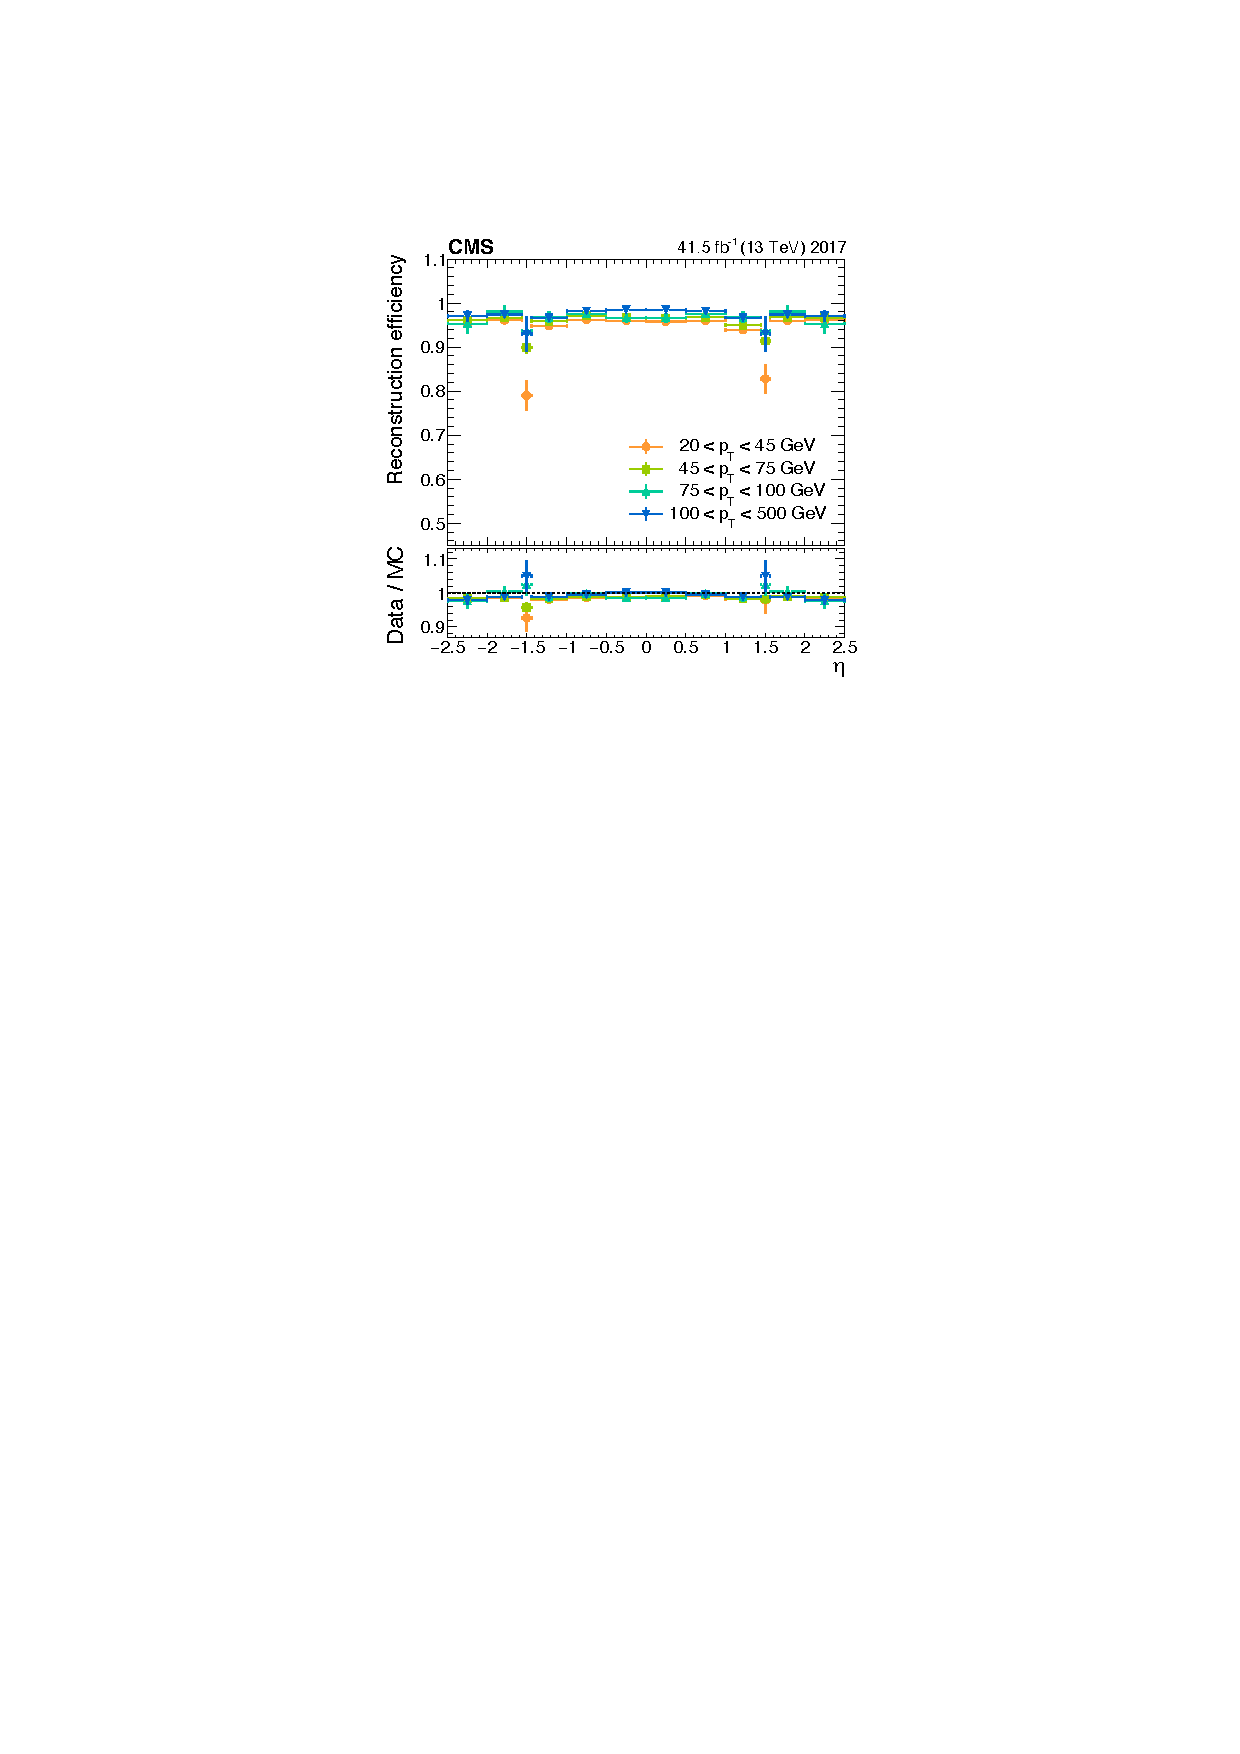
\includegraphics[width=0.55\textwidth]{figure/reco_el_eff.pdf}
    \caption[Electron reconstruction efficiency versus $\eta$ for the 2017 data.]
    {
        Electron reconstruction efficiency versus $\eta$ in data (upper panel) and data-to- simulation efficiency ratios (lower panel) for the 2017 data taking period. 
        The vertical bars on the markers represent the combined statistical and systematic uncertainties. 
        The region $1.44 < |\eta| < 1.57$ corresponds to the transition between the barrel and endcap regions of ECAL and is not considered in physics analyses.
    }
    \label{fig:reco_el_eff}
\end{figure}

\subsection{Electron identification and isolation}
The electron identification could be done by comparing the geometrical information, shape, and fitting properties between supercluster in the ECAL and track.
The isolation value is also defined similarly as Eq.~\ref{eq:reco_muon_iso}.

The $\Pe/\gamma$ physics object group defines the identification and isolation scheme with the following variables.
\begin{itemize}
    \item $\sigma_{|\eta|\eta}$: A spread of the ECAL supercluster in the $\eta$ direction.
        An electron from a hard process should have a narrow signature in the $\eta$ direction due to the occurrence of the bending radiation from electrons bending in the magnetic field.
    \item $|\Delta\eta|$ and $\Delta\Phi$: Geometric differences betwen the supercluster and the tracker.
    \item $H/E$: The ratio between the energy deposited in the HCAL and the ECAL in the super cluster region.
    \item $|\frac{1}{E}-\frac{1}{\rho}|$: Difference between the energy deposited in the supercluster and the track.
    \item $I_{\mathrm{PF,rel}}$ with EA: Isolation variable defined similarly to Eq.~\ref{eq:reco_muon_iso} with the effective areas.
    \item $d_{xy}$ and $d_z$: The impact parameters relative to a primary vertex.
    \item Missing hits in the tracker system.
    \item Whether the candidate passes the conversion veto cut.
\end{itemize}

The $\Pe/\gamma$ physics object group determines the exact cut values for each variable for different working points with different cut values for barrel and endcap electrons.
The cut values used in this analysis can be found in Tables~\ref{tab:reco_el_id_barrel} and~\ref{tab:reco_el_id_endcap}.


\begin{table}
    \caption[Electron identification and isolation cut values in barrel region.]
    {
        Electron identification and isolation cut values prescribed by the $\Pe/\gamma$ physics object group for barrel region $|\eta|<1.479$
    }
    \label{tab:reco_el_id_barrel}
    \centering\renewcommand\arraystretch{2.4}
    \resizebox{\textwidth}{!}{
        \begin{tabular}{|c|cccc|}
            \hline
            Variable & Veto & Loose & Medium & Tight \\
            \hline
            $\sigma_{|\eta|\eta} <$ & 0.0126 & 0.0112 & 0.0106 & 0.0104 \\
            $|\Delta\eta| <$                         & 0.00463 & 0.00377 & 0.0032 & 0.00255 \\
            $\Delta\Phi <$                          & 0.0148 &    0.0884 & 0.0547 & 0.022 \\
            $H/E < $  & $0.05+1.16/E_{\mathrm{SC}}+0.0324 \times \rho/E_{\mathrm{SC}}$ & $0.05+1.16/E_{\mathrm{SC}}+0.0324 \times \rho/E_{\mathrm{SC}}$ & $0.046+1.16/E_{\mathrm{SC}}+0.0324 \times \rho/E_{\mathrm{SC}}$ & $0.026+1.16/E_{\mathrm{SC}}+0.0324 \times \rho/E_{\mathrm{SC}}$ \\
            $I_{\mathrm{PF,rel}}$ with EA $<$ & $0.198+0.506/\PT$ & $0.112+0.506/\PT$ & $0.0478+0.506/\PT$ & $0.0287+0.506/\PT$ \\
            $1/E - 1/\rho <$ & 0.209 & 0.193 & 0.184 & 0.159 \\
            Missing inner hits $\leq$ & 2 & 1 & 1 & 1\\
            Pass conversion veto & Y & Y & Y & Y\\
            \hline
        \end{tabular}
    }
\end{table}

\begin{table}
    \caption[Electron identification and isolation cut values in endcap region.]
    {
        Electron identification and isolation cut values prescribed by the $\Pe/\gamma$ physics object group for endcap region $|\eta|>1.479$
    }
    \label{tab:reco_el_id_endcap}
    \centering\renewcommand\arraystretch{2.4}
    \resizebox{\textwidth}{!}{
        \begin{tabular}{|c|cccc|}
            \hline
            Variable & Veto & Loose & Medium & Tight \\
            \hline
            $\sigma_{|\eta|\eta} <$ & 0.0457 & 0.0425 & 0.0387 & 0.0353 \\
            $|\Delta\eta| <$        & 0.00814	& 0.00674	& 0.00632	& 0.00501\\
            $\Delta\Phi <$          & 0.19	& 0.169	& 0.0394 & 0.0236\\
            $H/E < $  & $0.05+2.54/E_{\mathrm{SC}}+0.183 \times \rho/E_{\mathrm{SC}}$ & $0.0441+2.54/E_{\mathrm{SC}}+0.0183 \times \rho/E_{\mathrm{SC}}$ & $0.0275+2.52/E_{\mathrm{SC}}+0.0183 \times \rho/E_{\mathrm{SC}}$ & $0.0188+2.06/E_{\mathrm{SC}}+0.183 \times \rho/E_{\mathrm{SC}}$ \\
            $I_{\mathrm{PF,rel}}$ with EA $<$ & $0.203+0.963/\PT$ & $0.108+0.963/\PT$ & $0.0658+0.963/\PT$ & $0.0445+0.963/\PT$ \\
            $1/E - 1/\rho <$ & 0.132 & 0.111 & 0.0721 & 0.0197 \\
            Missing inner hits $\leq$ & 3 & 1 & 1 & 1\\
            Pass conversion veto & Y & Y & Y & Y\\
            \hline
        \end{tabular}
    }
\end{table}
